\documentclass[12pt,a4paper]{article}
\usepackage[a4paper, margin=1in]{geometry}
\usepackage[utf8]{inputenc}
\usepackage[T1]{fontenc}
\usepackage{graphicx}
\usepackage{latexsym}
\usepackage{amsfonts,amssymb,amsmath,amsthm}
\usepackage{multirow}
\usepackage{multicol}
\setlength{\columnsep}{1.5cm}
\usepackage{setspace}
\usepackage{url}
\usepackage{array}
\usepackage{xfrac}
\usepackage{mwe}
\usepackage{tikz}
\usepackage{lmodern}
\usepackage{flowchart}
\usetikzlibrary{shapes,arrows,positioning,calc,fit}
\usepackage{graphics}
\usepackage{subfig}
\usepackage{booktabs}
\usepackage{float}
\usepackage{color,soul}
%\usepackage[numbers,sort&compress]{natbib}
\usepackage{hyperref}
%\usepackage{cite}
\usepackage{biblatex}
\addbibresource{References.bib}
\newcommand{\tom}[2]{{\color{red}{#1}}\footnote{\textit{\color{red}{#2}}}}
\newcommand{\ali}[2]{{\color{pink}{#1}}\footnote{\textit{\color{pink}{#2}}}}


\title{Thank You, Next}
\author{Ali M. Campbell\\
	Tom E.X. Miller}
\begin{document}
	\maketitle
	
	\section*{Abstract}

Mutualisms are among the most widespread species interactions with diverse and dynamic consequences.
Depending on environmental context the outcome of the interaction can range from parasitic to mutualistic. 
Most studies focus on a pair of species interacting in a mutualism, however most observed mutualistic interactions include more than two species. 
These are multi-species mutualisms, where there are multiple partners interacting with the same focal species. 
\hl{The partners can directly impact the focal species through the interactions, \tom{and indirectly impact them through interactions with each other}{***This is true but not something we are well poised to address with our data so might be risky to bring it up.***}. }
The cactus \textit{Cylindriopuntia imbricata} reward partners with extrafloral nectar in exchange for defense by various ant species (primarily \textit{Crematogaster opuntiae} and \textit{Liometopum apiculatum}, though there are many other ant species with smaller populations) from herbivores and seed predators. 
\hl{Using a 20-year collection of demographic data (growth, survival, reproduction, ant partners, herbivory, etc.) from these cacti in New Mexico, we estimate the fitness of the cacti populations with every combination of partners, allowing us to *** understand what accounts for partner diversity in this system *** understand if the current partner diversity of the system is associated with the optimal fitness *** and the impacts of these partners on different vital plant processes across their life history (such as partner impacts on reproduction, survival, or growth). }
We found that different ant partners had different impacts on cacti vital rates suggesting there may be a different 'best' partner during pre-reprodctive life stages than during reproductive life stages, and that the highest cacti fitness is associated with the current partner set (all possible ant partners are available).
Together, these results suggest that complementarity may account for the benefits that these plants experience with partner diversity. 
Our results demonstrate the importance of evaluating a mutualism within a community context and \tom{suggest that even slight differences of rewards between mutualist partners can help promote fitness of the cacti}{Nothing you have reported in the abstract so far really supports this statement.}. 

\tom{Each of the ant partners}{Again, abstract should briefly state how many and which.} in this system are within the same guild, all offering defense from herbivores, \tom{with only one ant species interacting with each individual cactus in a given period of time}{Redundant with statement above.}. 
Though these ants may offer very similar rewards, \tom{they likely differ in some way}{Vague}. 
Two possible ways they could differ are the \tom{fitness boost}{Vague and too colloquial.} they offer the focal species or the \tom{period of ontogeny}{We have size structure data but we are not really dealing with ontogeny per se, so I think it is safer to discuss things in terms of size.} in which they offer the greatest fitness boost. 
\tom{Using a long-term data-set, we show that there are differences in the impacts of different ant partners on various vital rates of the cacti across ontogeny. Our results demonstrate the importance of evaluating a mutualism within a community context and suggest that even slight differences of rewards between mutualist partners can help promote fitness of the cacti. }{I am a little confused - maybe these two paragraphs are two different versions of the abstract?}
\tom{}{I know this was just a first stab at the abstract, and written when you don't yet have your final results. But eventually this will need to be tightened up and edited to better describe the conceptual motivation, what was done, and what was found.}

\section*{Context/Introduction}
BASELINE OF MUTUALISMS
Mutualisms are species interactions in which all involved participants benefit. They are among the most widespread species interactions\cite{Chamberlain2014,Stachowicz2005,BoucherDouglasH.1985} with diverse and dynamic consequences. 
\ali{The benefits from these interactions are called rewards, but they require investment of resources into the interaction}{I'm honestly not sure if I need to explain this idea? Do I need to include more basic mutualism background? I have tried to shift this so that I cover a small amount and then jump into the idea of partner diversity in mutualisms instead}. 

Historically, scientists focused on pairwise mutualisms\cite{Bascompote2019}, however, in recent years multi-species mutualisms have been more heavily studied. 
It has become apparent that partner diversity in mutualisms often leads to non-additive fitness benefits for the focal mutualist\cite{Afkhami2014, Palmer2010}. 
This means the benefits can be greater than, less than, or equal to the sum of the benefits observed in each of the pairwise interactions with the focal mutualist that makes up the multi-species mutualism. 
This is true for many complicated reasons, including interactions between the various partners, niche overlap, temporal resource variation, and differences in partner quality, functional benefit, and competitive ability\cite{stanton2013, Afkhami2014,Boucher1982}.
Often partners have similar resource needs, particularly if they are in the same guild, which can lead to resource competition and fighting, potentially reducing benefits, or to increased quality and frequency of benefits\cite{Bascompote2019,Stanton2003}.
For this reason, pairwise studies cannot be accurately used to predict the outcomes of multi-species mutualisms\cite{Palmer2010, Stanton2013. Chamberlain2014, Song2020} which are more common.
\ali{***** Biodiversity ecosystem function? }{After this I feel like I go straight into the mechanisms which explain the potential positive effects of diversity, but I don't specify that I am talking about those and I also don't talk about any explainations of negative effects? Maybe if I include the connection between BEF theory and mutualisms here it will make a nice bridge to the benefits of diversity?} 
Observational studies on the effects of diverse multi-species mutualism systems are necessary to help us understand the demographic effects of partner diversity in mutualisms. 


The diversity of partners in a multi-species mutualism causes varied demographic effects on the population of the focal mutualist which can be explained by a number of mechanisms.
Partners can vary in many ways: in some cases, the quality varies leading to some true mutualist partners, some freeloaders, and even some parasites\{Bronstein1994, Afkhami2014,Song2020,West2007,Frederickson2013}; in other cases, the function of the partner can vary, each offering a different type of reward to the focal mutualist \{Stanton2003}.
Partner quality variations can remain consistent across years and life stages of the focal mutualist or they can shift year to year. 
When partner quality remains consistent across time, meaning one partner is always better or worse than another, the effects of partner diversity on the focal mutualist can be explained by a mechanism called sampling effect.
This is the concept that if partners vary in quality, then a more diverse sample of the partner community may be more likely to include the ``best" one\cite{Batstone2018}.
When a focal mutualist in a multi-species mutualism \ali{experiences}{not sure if this is the right word} sampling effect the fitness of that focal mutualist should be equal to the fitness of the focal mutualist if they interacted only with the ``best" partner. 
In some cases the quality of partners is not constant, rather it varies year to year due to environmental limitations, such as resource shortages and niche shifts.
The effects of partner diversity in these systems can be explained by the portfolio effect, the idea that each partner is the ``best" under a different set of conditions, which vary temporally\cite{Winfree2020,Batstone2018}. 
This mechanism works almost like a financial portfolio, when one partner has a bad year another partner has a good year, meaning the overall fitness benefits of the interactions remain relatively constant across temporal variation\cite{Batstone2018}.
Finally, partners can vary functionally, meaning each partner offers a different type of reward to the focal mutualist. 
The effects of partner functional diversity can be explained by the mechanism complementarity, the idea that each partner may account for some part of the benefits, but each has different functional pathways, which together can aid in broader benefits\cite{Winfree2020,Batstone2018}.
This variation can be both within and outside of a guild, meaning the variation can be very large, such as the difference between pollination and defense among other functions\cite{Bronstein2006}, or relatively small, such as similar rewards across different life stages\{Stanton2003}. 
Complementarity in a system is evidenced by synergistic benefits, meaning the fitness of the focal mutualist is higher than the fitness if the focal mutualist interacted with any one ``best" partner\{Batstone2018}. 
\ali{These three mechanism could explain the positive partner diversity effects on a focal mutualist in a multi-species mutualism, if these benefits exist.}{I am struggling on the transition between this paragraph and the next.}
 
Multi-species mutualisms are a huge group of interactions which vary considerably. 
While there are many types of mutualistic interactions, including pollination, defense, dispersal, housing, and many more\cite{Bronstein2006} in this paper we will focus on defensive ant-plant mutualisms.
These involve plants which provide extra-floral nectar and/or ``housing'' to ants which in turn defend them from herbivores\cite{Bronstein1998}. 
While these interactions have been well studied\cite{} in the literature, few have considered how diversity within ant defender guilds affect the overall benefits of mutualism for the plant partner. 

This study focuses on the long lived \textit{Cylindriopuntia imbricata} (tree cholla) and its ant mutualists. 
Tree cholla have a range which extends across the Southwest United States into Northern Mexico, with our study area set in New Mexico, US at the Sevilleta LTER.
These cacti flower in the spring throughout the summer, their reproductive season, outside of which they are not tended by ants. 
During the reproductive season these plants experience increased visitation by seed predators and herbivores, which influence their reproductive outputs, survival, growth, etc.
There are a number of observed ant partners which interact with the cacti in this part of their range, including \textit{Crematogaster opuntiae} (\textit{Crem.}), \textit{Liometopum apiculatum} (\textit{Liom.}), \textit{Forelius pruinosus}, an unidentified \textit{Camponotus} species, an unidentified \textit{Phenogaster} species, among others. 
The ants which most commonly interact with the cacti are \textit{Liom.} and \textit{Crem.}, while others are seen with low enough frequency that for the purpose of this paper we refer to them as ``other" ants. 
These ant partners are all in the same guild, meaning they all provide denfense to the cacti from insect herbivores and seed predators in return for extrafloral nectar (EFN).
The cacti in this mutualism are each tended by one species at a time, for their entire reproductive season with little turnover until the winter between reproductive seasons. 
Some of the ant partners are more effective defenders than others, with \textit{Liom.} tended reproducing plants experiencing the lowest level of herbivory as shown in Figure \ref{fig:herb}.
This shows that although all the ants associated with the tree cholla are within one guild, they are not all equal and may have different demographic effects on the cacti.

In this paper we will answer a number of questions about the demographic effects of partner diversity in multi-species mutualisms:
\begin{enumerate}
  \item{What are the contrasting demographic effects of multiple partners?}
  \item{What combination of ant partners is associated with the highest fitness for the tree cholla?}
  item{What mechanisms explain the effects of multiple ant partners on the tree cholla?}
\end{enumerate}

To answer these questions we used a long-term dataset of demographic information (size, survival, number of flowers produced or aborted, etc.) and ant partner data (species, number of ants) to track the structure of the population across time as well as individual level impacts of ant partners on the cacti. 
We analyzed the impacts of partner diversity on each individual vital rate (survivial, growth, floral-viability, etc.) with bayesian models, which we used to parameterize an Integral Projection Model (IPM).
With the IPM we moved beyond what has been done in previous studies\cite{Palmer2010} to identify which mechanisms explain the effects of partner diversity on the tree cholla. 


We hypothesized that the cacti would experience the highest fitness when interacting with all partners observed in the field, meaning the current mutualism results in the highest fitness for the cacti.
We also hypothesized that complementarity would explain these positive effects of partner diversity in the multi-species mutualism.
\section*{Methods}
\subsection*{Study System}

To determine how interactions with multiple partners impacts the cacti over time, we have monitored a population of Cholla cacti annually since 2004. 
This study was conducted in the Los Pinos mountains, a small mountain chain located on the Sevilleta National Wildlife Refuge, a Long-term Ecological Research (LTER) site in central New Mexico. 
The tree cholla cacti are common in high Chihuahuan desert habitats, with their native range spanning the southwestern USA *** Benson 1982***. 
These arborescent cacti produce new cylindrical segments every year which develop either into fruits which produce seeds or into vegetative segments with large spine which increase the size of the cactus %***Miller, Tenhumberg \& Louda 2008***. 
In central New Mexico, vegetative growth occurs from May -- August.

Cholla cacti secrete extra-floral nectar (EFN) from glands on young vegetative segments and reproductive segments. 
\tom{This extra-floral nectar varies in chemical makeup across the lifespan of the cactus *** Miller ??***. }{This is pretty vague, so if you are going to say this you should add more detail.}
At the Sevilleta, the cacti are visited by \tom{multiple species}{I think it would be better to say primarily two species plus other rare species, and giving the frequencies} of ground-nesting ants, \textit{Crematogaster opuntiae}, \textit{Liometopum apiculatum}, and \tom{many other species}{which ones?} which occur at \tom{small}{low} frequencies. 
These ants are attracted to the EFN and in return fight off the \tom{seed predators}{which ones?} \tom{which also visit the cacti}{An example of words that make sentences clunky without adding any information}. 
These ants never co-occur on the same plant, \tom{instead competing for plant services}{This is a hypothesis, not something that has been demonstrated.}. 
\tom{Over the lifetime of the cacti each plant interacts with multiple partners as they tend to switch out season to season.}{I would guess that most plants do not have much switching. I think you also need to talk about vacancy and the start of EFN production at larger reproductive sizes, more detail on transitions in ant state between vs within years. All of this should be in a separate subsection about natural history.}

\tom{There}{This paragraph should also be in a natural history subsection and obviously needs more detail. See my earlier papers and references therein and let me know if you have specific questions.} are a variety of insect herbivores and seed predators which attack the cacti, focusing either on the vegetative segments and the reproductive segments. 
There are a number of insects which occur commonly on these cacti at the Sevilleta. 
These include the weevil, the NP, and the *** (I think there is a moth as well?). 
The \tom{weevil}{what species?} feeds on ***. 
The NP feeds on ***. 
Finally, the moth?? feeds on ***. 
All of these predators can have significant impacts on the fitness of both individual cacti and the population. *** Miller 2009***. 

\tom{The}{This should be a subsection for data collection, with significantly more information than what you have here so that the methods could be reproduced.} data collected on these cacti are from an \tom{18-year}{Which years?} data-set. 
There are 8 30 $\times$ 30 meter plots from which this data is taken. 
Each plot is \tom{surveyed}{what does this mean?}, and each plant within each plot is tagged and \tom{logged}{what does this mean} each year. 
For every plant we take data on their survival, \tom{size}{how is size measured?}, \tom{ant state}{what is this?}, \tom{herbivore presence}{this makes it sounds like presence/absence which is not what we record}, \tom{flowering data}{what does this mean?}, and \tom{seed data}{what does this mean?}. 
\tom{This allows us to track the progression of individual plants across many years.}{No new information here.} 
The length of this data-set 

\subsection*{Statistical Modeling}
To understand the impacts of multiple species interactions on the cacti populations, we constructed \tom{bayesian demographic models of many vital rates}{What are bayesian demographic models? WHat are the many vital rates?}. 
With these models, we were able to ask (i) Do the impacts of ant presence on \tom{cacti fitness}{these models are not measuring fitness} differ across ant species? (ii) What are the probabilities of an individual cactus interacting with each ant species?.\tom{}{I think it's good that you have these as separate questions but I think each one needs a lot more context and detail.} 

The vital rates of the cacti considered in this model include survival rate, growth rate, reproductive state, floral abortion rate, \tom{seed production, and germination}{You have not described where these data come from.}. 
\tom{We fit generalized linear mixed effects models in a heirarchical Bayesian framework to quantify each of the vital rates.}{Not a reproducible description of the methods. e.g., what distributions were used, what were the fixed and random effects, which models included ant effects, what were the priors, how many chain and iterations, and were convergence and fit assessed, etc?} 
\tom{Each model takes the data from year \textit{t} and estimates the values in year \textit{t+1}.}{This is true only for growth and survival.} 
This allows us to predict a vital rate for any plant with a given set of characteristics, \tom{such as size and ant state}{Not such as, it is really just these two things.}. 
\vspace{1cm}

	\subsection*{Demographic Modeling}

The statistical models described above parameterize the Integral Projection Model (IPM) that we used to estimate population growth under various partner conditions.  
This model was used to estimate the growth rate of the cactus population, effectively a quantitative measure of the fitness of the population. 
The fitness was estimated under the \tom{range of all different conditions, no ants present, one ant species present, two ant species present, all ant species present.
These allow us to compare the fitness of the cacti under no mutualistic interactions, pairwise mutualisms, and various multi-species mutualisms to show which case results in the highest fitness for the cacti.}{This needs a more thorough explanation, but I would also do this later after the model has been introduced and explained.} 

Following previous studies, we modeled the life cycle of \textit{C. imbricata} using continuously size-structured plants,$n_i(x)$, and two discrete seed banks ($\beta_{1,t}$ and $\beta_{2,t}$) corresponding to 1 and 2-year old seeds.
$$
B_{1, t+1} = \kappa \delta \sum_{i}^{4} \int_L^U P(x) A_i(x) F(x)n_i(x) dx \\
$$
$$
B_{2,t+1} =  (1 - \gamma_1)B_{1,t}\\
$$

The functions $P$, $F$, and $A$ give the probability of flowering, the number of flowerbuds produced, and the proportion of flowerbuds which will create seeds. 
Each of these functions, estimated by a Bayesian model calculates these values for an $x$-sized plant in year $t$. 
The proportion of flowerbuds which will produce seeds ($A$) is also dependent on the ant species present on the plant $i$ in year $t$. 
The integral is multiplied by the number of seeds per fruit ($\kappa$) and the probability of seed dispersal/survival ($\delta$) to give the number of seeds that enter the 1-year old seed bank. 
Parameters $U$ and $L$ are the upper and lower  bounds, respectively, of the plant size distribution. 
Plants can recruit out of the 1-year seed bank with the probability of $\gamma_1$ or transition to the 2-year seed bank with a probability of $1 - \gamma_1$. 
Seeds in the 2-year seed bank are assumed to either germinate with a probability of $\gamma_2$ or die. 

The size dynamics of the plants are given by:

$$
n(y,i)_{t+1} = (\gamma_1 B_{1,t} + \gamma_2 B_{2,t}) \eta(y) \omega \beta_i  + \\
$$
$$
\sum_{j}^{4} \int_L^U S_j(x) G_j(y,x) \tau_{ij}(x) n_j(x) dx \\
$$

The final equation gives the \tom{size}{not just population size but also composition in terms of size and ant state - this needs to be explained better} of the \textit{C. imbracata} population $n$ in year $t+1$ based on the vital rates and size $n$ of the population in year $t$.
The first term gives the recruitment from 1 and 2-year seedbanks to size $y$.
$\eta(y)$ gives the seedling size distribution, which is assumed to be normally distributed, and $\omega$ gives the proportion of seedlings which survive from germination (late summer) to the census (May). 
The second term gives the changes in the population of the cacti which are not recruits. 
The functions $S$ and $G$ give the probabilities of surviving from year $t$ to $t+1$ and growing to size $y$ from year $t$ to year $t+1$, respectively. 
Each depends on the size $x$ in year $t$ and the ant state $j$ in year $t+1$. 
Finally, $\tau_{ij}$ is the probability of a cactus which is size $x$ with ant partner $i$ in year $t$ being tended by ant partner $j$ in year $t+1$. 

 \subsection*{Model analysis}

\textbf{TOM STOPPED EDITING HERE}

\section*{Results}
\subsection*{Vital Rates}

We used field data on cholla cacti to evaluate the differing impacts that the ant mutualism has on the fitness of the cacti. The fitness can be broken down into a number of vital rate components, including survival, growth, probability of flowering, number of fruits and seeds produced, etc. called vital rates. We found that many of these vital rates differ in the presence of different ant species. 


\begin{figure}[!ht]
	\centering
	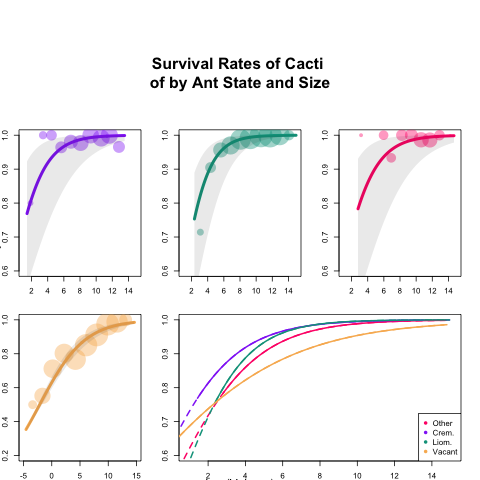
\includegraphics[width = 0.85\linewidth]{Figures/surv_panels_cropped.png}
	\caption{Probability of cactus survival from year t to year t+1 when tended by (a) \textit{Crem.} (Purple), (b) \textit{Liom.} (Teal), (c) ants in the other category (Pink), or (d) no ants (Yellow). Panels (a-d) show the best-fit line estimating the survival probabilities of cacti, with a grey area representing the uncertainty, and circles representing the actual data (scaled to represent number of observations). (e) shows the best-fit probabilities of survival of different-sized cacti with all ant partners.}
	\label{fig:surv}
\end{figure}

	The first vital rate we analyzed was the survival of the cacti. As you can see in Figure \ref{fig:surv}, the survival rate of cacti vary significantly across their lifetimes as they grow. Young (small) cacti have relatively low survival rates, near $30\%$ while the older mature cacti have much higher survival rates, near $100\%$. This means cacti are at their most vulnerable to death when they are young. The survival rates differ with more than just the size of the cacti, the ant species present on the cactus is also important. 

There are no very small cacti tended by ant partners because they do not produce EFN. This is reflected in Figure \ref{fig:surv} where only the vacant data (yellow) in panel (d) extends to the smallest sizes. Once cacti reach a size large enough to attract ant partners with EFN, the cacti which are partnered with \textit{Crem.} have the highest survival rates compared to all other cacti. When the cacti reach their larger sizes, the partnered plants all reach a nearly $100\%$ survival rate while plants with no partners have a slightly lower survival rate for all large cacti. This result indicates that \textit{Crem.} tended plants may have an advantage, when they are relatively small, over other cacti. 

The next vital rate we analyzed was the viability rate of the cacti, the proportion of fruits produced which are viable for reproduction. It is clear from Figure \ref{fig:viab} that the cacti tended by \textit{Liom.} ants experience significantly higher proportions of viable fruits. This result aligns with much of the literature which shows that \textit{Liom.} are more aggressive against herbivores and seed predators, therefore are very high quality defenders. This high-quality defense is imperative for high viability rates on reproducing cacti which are likely to attract many antagonists due to the quality of their EFN. 


\begin{figure}[!ht]
	\centering
	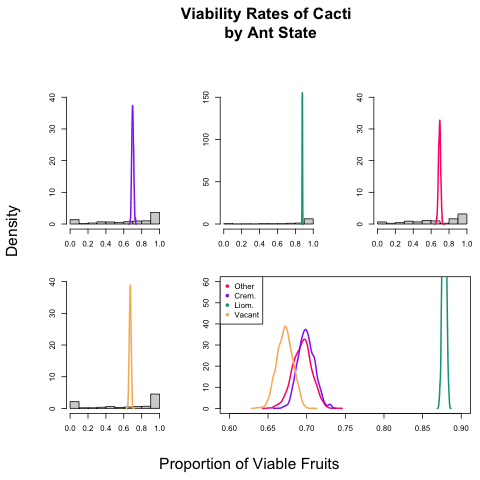
\includegraphics{Figures/viab_hist.png}
	\caption{Proportion of viable fruits produced by a cactus in year t+1 when tended in year t by (a) \textit{Crem.} (Purple), (b) \textit{Liom.} (Teal), (c) ants in the other category (Pink), or (d) no ants (Yellow). Each panel (a-d) shows a histogram of the actual data overlayed with a density distribution of the predicted viability rate of the cacti. Panel (e) shows the predicted distributions of viability rates separated by ant species.}
	\label{fig:viab}
\end{figure}

A third vital rate considered in this paper is the growth rate. Cacti who are attacked by herbivores are likely to lose sections of their growth, leading to a lower, or even negative, growth rate. In Figure \ref{fig:grow} you can clearly see that untended plants are the only cacti which experience a negative growth rate at any size. This again aligns with expectations that tended cacti are being defended from herbivores and are therefore unlikely to lose enough vegetation to result in a negative growth rate. 

\begin{figure}[!ht]
	\centering
	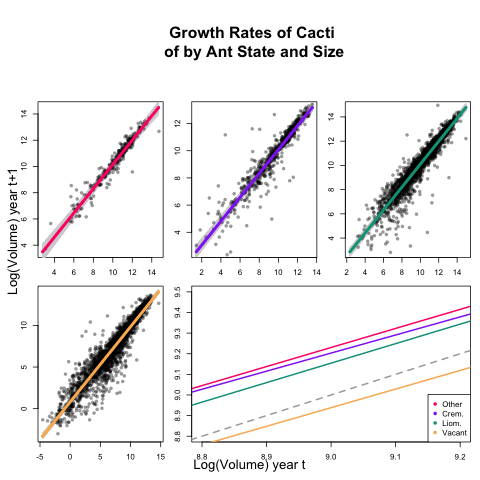
\includegraphics{Figures/grow_panel.png}
	\caption{The size of a cactus in year t+1 given a previous size in year t and being tended by (a) \textit{Crem.} (Purple), (b) \textit{Liom.} (Teal), (c) ants in the other category (Pink), or (d) no ants (Yellow). Each panel (a-d) shows a best-fit prediction of the future size based on the previous size, the uncertainty in grey surrounding the best-fit, and the actual data in (circles scaled to represent the number of observations). Panel (e) shows all best-fit lines together in the same colors as above and a line (grey, dashed) above which plants are growing (have a positive growth rate) and below which plants have a negative growth rate.}
	\label{fig:grow}
\end{figure}

\begin{figure}[!ht]
	\centering
	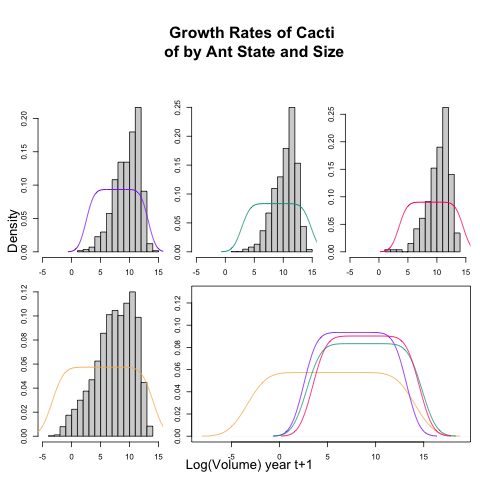
\includegraphics{Figures/grow_dist_panel2.png}
	\caption{The size of a cactus in year t+1 given a previous size in year t and being tended by (a) \textit{Crem.} (Purple), (b) \textit{Liom.} (Teal), (c) ants in the other category (Pink), or (d) no ants (Yellow). Each panel (a-d) shows a distribution of the predicted future size based on the previous sizeand a histogram of the actual data. Panel (e) shows all predicted distributions together in the same colors as above.}
	\label{fig:grow2}
\end{figure}

	\subsection*{Ant Transition Rates}

In addition to the vital rates of the cacti, we also analyzed the transition rates from one ant partner to another across years. 

\begin{table}[]
	\centering
	\begin{tabular}{|p{0.25 \linewidth}   |p{0.25 \linewidth}|p{0.25 \linewidth}|}
		\hline
		\textbf{Ant States Possible} & \textbf{Growth Rate ($\frac{n_{t+1}}{n_t}$)} & \textbf{Population $\lambda$}\\
		\hline
		No ants & &\\
		\hline
		\textit{Liom.} & & \\
		\hline
		\textit{Crem.}  & & \\
		\hline
		Other & & \\
		\hline
		\textit{Liom.} \& \textit{Crem.} & & \\
		\hline
		\textit{Liom.} \& Other & & \\
		\hline 
		\textit{Crem.} \& Other & & \\
		\hline
		\textit{Liom.}, \textit{Crem.} \& Other & & \\
		\hline
	\end{tabular}
	\caption{Caption}
	\label{tab:table_sims}
\end{table}
%	\begin{multicols}{2}

\section*{Discussion}

There is a constant tension within life cycles between energy and resource allocation. Individuals often have the ability to either put significant resources towards one process or split their resources between multiple. Full energy allocation to one process generally means better results, but splitting resources is a form of bet hedging ***. The cacti studied here experience a certain tension between their many vital rates, particularly growth and reproduction because each year they produce new floral buds and new vegetative growth. Small plants rarely put out flowers and instead focus on growth, but larger plants must choose each year. The analyses of the individual vital rates indicate that different ant species may protect different processes better than others. In particular \textit{Crem.} may offer advantages to smaller plants by protecting their new vegetation well. This is seen in the higher survival rates and growth rates of small and medium cacti with \textit{Crem.} tenders in Figure \ref{fig:grow} and Figure \ref{fig:surv}. \textit{Liom.} ants alternatively may protect reproductive focus more than other partners. The \textit{Crem.} tended plants however, have lower viability rates than any other ant tended plants, indicating they do not protect flowers well from herbivores(Figure \ref{fig:viab}). This is seen in Figure \ref{fig:viab} where it is shown that plants tended by \textit{Liom.} have the highest viability rates of their flowers, resulting in higher pollination rates. Larger plants are also less likely to lose branches when they are tended by \textit{Liom.} (Figure \ref{fig:grow}), keeping them healthy and more able to generate new plants. Each of these ants individually offer both benefits and drawbacks but considered together may indicate complementarity across ontogeny. 
	
\end{document}

\typeout{\bibliography{References.bib}}